%% LyX 2.1.4 created this file.  For more info, see http://www.lyx.org/.
%% Do not edit unless you really know what you are doing.
\documentclass[11pt,czech,american]{book}
\usepackage[T1]{fontenc}
\usepackage[utf8]{inputenc}
\usepackage[a4paper]{geometry}
\geometry{verbose,tmargin=4cm,bmargin=3cm,lmargin=3cm,rmargin=2cm,headheight=0.8cm,headsep=1cm,footskip=0.5cm}
\pagestyle{headings}
\setcounter{secnumdepth}{3}
\usepackage{url}
\usepackage{amsmath}
\usepackage{amsthm}
\usepackage{amssymb}
\usepackage{graphicx}
\usepackage{setspace}
\usepackage[final]{pdfpages}
\usepackage{natbib}
\usepackage{mathrsfs}
\usepackage{algorithm}
\usepackage{algorithmicx}
\usepackage[noend]{algpseudocode}
\usepackage{caption}

\usepackage{array}
\usepackage{ragged2e}

\usepackage{lipsum}
\usepackage{psvectorian}

\makeatletter
%%%%%%%%%%%%%%%%%%%%%%%%%%%%%% Textclass specific LaTeX commands.
\newenvironment{lyxlist}[1]
{\begin{list}{}
{\settowidth{\labelwidth}{#1}
 \setlength{\leftmargin}{\labelwidth}
 \addtolength{\leftmargin}{\labelsep}
 \renewcommand{\makelabel}[1]{##1\hfil}}}
{\end{list}}

%%%%%%%%%%%%%%%%%%%%%%%%%%%%%% User specified LaTeX commands.
%% Font setup: please leave the LyX font settings all set to 'default'
%% if you want to use any of these packages:

%% Use Times New Roman font for text and Belleek font for math
%% Please make sure that the 'esint' package is turned off in the
%% 'Math options' page.
\usepackage[varg]{txfonts}

%% Use Utopia text with Fourier-GUTenberg math
%\usepackage{fourier}

%% Bitstream Charter text with Math Design math
%\usepackage[charter]{mathdesign}

%%---------------------------------------------------------------------

%% Make the multiline figure/table captions indent so that the second
%% line "hangs" right below the first one.
%\usepackage[format=hang]{caption}

%% Indent even the first paragraph in each section
\usepackage{indentfirst}

%%---------------------------------------------------------------------

%% Disable page numbers in the TOC. LOF, LOT (TOC automatically
%% adds \thispagestyle{chapter} if not overriden
%\addtocontents{toc}{\protect\thispagestyle{empty}}
%\addtocontents{lof}{\protect\thispagestyle{empty}}
%\addtocontents{lot}{\protect\thispagestyle{empty}}

%% Shifts the top line of the TOC (not the title) 1cm upwards 
%% so that the whole TOC fits on 1 page. Additional page size
%% adjustment is performed at the point where the TOC
%% is inserted.
%\addtocontents{toc}{\protect\vspace{-1cm}}

%%---------------------------------------------------------------------

% completely avoid orphans (first lines of a new paragraph on the bottom of a page)
\clubpenalty=9500

% completely avoid widows (last lines of paragraph on a new page)
\widowpenalty=9500

% disable hyphenation of acronyms
\hyphenation{CDFA HARDI HiPPIES IKEM InterTrack MEGIDDO MIMD MPFA DICOM ASCLEPIOS MedInria}

%%---------------------------------------------------------------------

%% Print out all vectors in bold type instead of printing an arrow above them
\renewcommand{\vec}[1]{\boldsymbol{#1}}

% Replace standard \cite by the parenthetical variant \citep
%\renewcommand{\cite}{\citep}

\makeatother

\usepackage{babel}

\newcommand{\ornamentleft}{%
	\psvectorian[width=2em]{2}%
}
\newcommand{\ornamentright}{%
	\psvectorian[width=2em,mirror]{2}%
}

\newcommand{\ornamentheader}[1]{%
	\begin{center}
		\ornamentleft
		\quad{\large\emph{#1}}\quad % style as desired
		\ornamentright
	\end{center}%
}

\newlength{\rlength}\setlength{\rlength}{16cm}
\newcommand{\ruletext}[2][\rlength]{%
	\noindent%
	\parbox{#1}{%
		\noindent\dotfill\raisebox{-.3\ht\strutbox}{#2}\dotfill\par}%
}





\begin{document}
\def\documentdate{July 7, 2017}

\newtheorem{definition}{Definition}[chapter]
\newtheorem{note}{Note}[chapter]
\newtheorem{example}{Example} 
\newtheorem{assumption}{Assumption} 

\newtheorem{theorem}{Theorem}

\captionsetup[figure]{labelfont={bf},labelformat={default},labelsep=period,name={Fig.}}


\def\documentdate{\today}

\pagestyle{empty}
{\centering

\noindent %
\begin{minipage}[c]{3cm}%
\noindent \begin{center}

\includegraphics[width=3cm,height=3cm,keepaspectratio]{Images/TITLE/cvut}
\par\end{center}%
\end{minipage}%
\begin{minipage}[c]{0.6\linewidth}%
\begin{center}
\textsc{\large{}Czech Technical University in Prague}{\large{}}\\
{\large{}Faculty of Nuclear Sciences and Physical Engineering}
\par\end{center}%
\end{minipage}%
\begin{minipage}[c]{3cm}%
\noindent \begin{center}

\includegraphics[width=3cm,height=3cm,keepaspectratio]{Images/TITLE/fjfi}
\par\end{center}%
\end{minipage}

\vspace{3cm}


\textbf{\huge{}Real Options Valuation: A Dynamic Programming Approach}{\huge \par}

\vspace{1cm}


\selectlanguage{czech}%
\textbf{\huge{}Oceňování projektů metodou reálných opcí z pohledu dynamického progamování}{\huge \par}

\selectlanguage{american}%
\vspace{2cm}


{\large{}Master's Thesis}{\large \par}

}

\vfill{}

\begin{lyxlist}{MMMMMMMMM}
\begin{singlespace}
\item [{Author:}] \textbf{Filip Rolenec}
\item [{Supervisor:}] \textbf{Ing. Rudolf Kulhavý, DrSc.}
\end{singlespace}

\item [{Language~advisor:}] \textbf{Ing. Rudolf Kulhavý, DrSc.} 
\begin{singlespace}
\item [{Academic~year:}] 2020/2021\end{singlespace}

\end{lyxlist}
\newpage{}

~\newpage{}

~

\vfill{}


\begin{center}
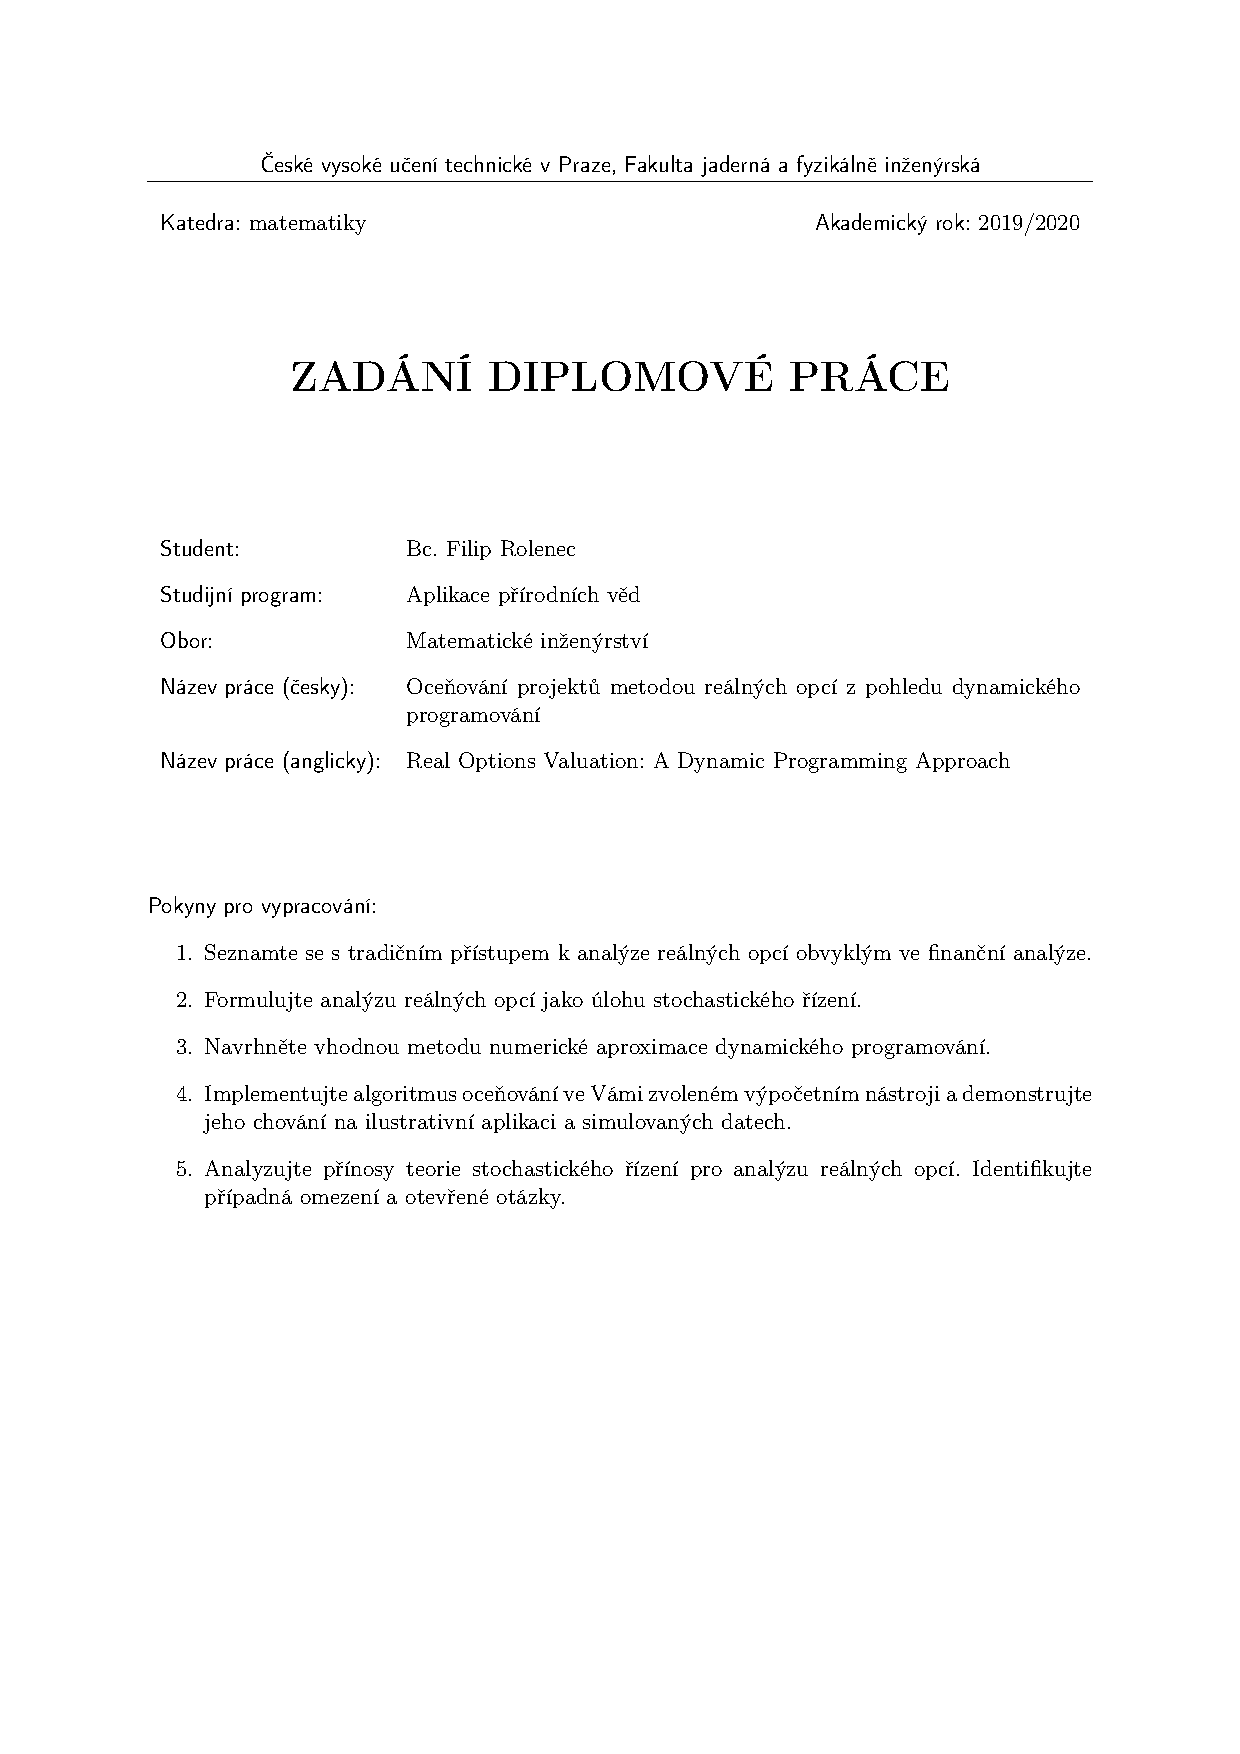
\includepdf[pages={1}]{Images/zadaniMT.pdf}


\par\end{center}

\vfill{}


~\newpage{}

~

\vfill{}


\begin{center}
\includepdf[pages={2}]{Images/zadaniMT.pdf}
\par\end{center}

\vfill{}


~\newpage{}

\noindent \emph{\Large{}Acknowledgment:}{\Large \par}

\noindent I would like to thank my supervisor Ing. Rudolf Kulhavý, DrSc. for his professional guidance and all the advice given while creating this thesis. 

\vfill

\noindent \emph{\Large{}Author's declaration:}{\Large \par}

\noindent I declare that this Master's thesis is entirely
my own work and I have listed all the used sources in the bibliography.

\bigskip{}


\noindent Prague, \documentdate\hfill{}Filip Rolenec

\vspace{2cm}


\newpage{}

~\newpage{}

\selectlanguage{czech}%
\begin{onehalfspace}
\noindent \emph{Název práce:}

\noindent \textbf{Oceňování projektů metodou reálných opcí z pohledu dynamického progamování}
\end{onehalfspace}

\bigskip{}


\noindent \emph{Autor:} Filip Rolenec

\bigskip{}


\noindent \emph{Obor:} Matematické inženýrství 


\bigskip{}


\noindent \emph{Druh práce:} Diplomová práce

\bigskip{}


\noindent \emph{Vedoucí práce:} Ing. Rudolf Kulhavý, DrSc.


\bigskip{}


\noindent \emph{Abstrakt:} Oceňování převážné většiny investičních příležitostí se dnes stále určuje metodou \textit{diskontovaných peněžních toků} (DCF) \ref{}. DCF metoda je přímočará a pro jednoduché projekty dává velmi přesné výsledky. Složitější projekty, které pro tuto práci definujme jako projekty s vysokou mírou vnitřní neurčitosti a existencí manažerských rozhodnutí značně ovlivňujících strukturu projektu (reálné opce), jsou dnes oceňovány metodou \textit{real option analysis} (ROA). Metoda ROA přiznává hodnotu možnostem změny projektového plánu, v důsledku čehož je ohodnocení ROA vyšší než DCF. 

Tato práce má za cíl interpretovat řízení projektů a s ním související ocenění, jako řízení stochastického systému. Rozsáhlá teorie stochastického řízení \ref{}, \ref{}, \ref{}, dovoluje vybudovat novou teorii oceňování postavenou na základech ROA, která mimo jiné řeší omezení ROA na pouze jediný zdroj neurčitosti - například cenu těžených minerálů na trhu \cite{}. 

Nový originální přístup k oceňování projektů, který kombinuje dosavadní dosažené znalosti v ekonomické teorii (ROA) a teorii stochastického řízení systémů (SDT) je obecně definován v první části práce a prakticky otestován simulacemi na třídě problémů z oblasti  <Area of study>. 

Simulace ukazují, že kromě lepší interpretovatelnosti modelu a možnosti vložení subjektivních pravděpodobností je ocenění metodou ... přesnější o ... \%. Výsledky vyjadřují naději na zvýšenou adopci metody ... v praxi. 


\bigskip{}


\noindent \emph{Klíčová slova:}   Analýza reálných opcí, Diskontované peněžní toky, Oceňování projektů, Stochastické řízení, Těžební průmysl



\selectlanguage{american}%
\vfill{}
~

\begin{onehalfspace}
\noindent \emph{Title:}

\noindent \textbf{Real Options Valuation: A Dynamic Programming Approach}
\end{onehalfspace}

\bigskip{}


\noindent \emph{Author:} Filip Rolenec

\bigskip{}


\noindent \emph{Abstract:} The valuation of investment opportunities (projects) is nowadays still predominantly computed by the\textit{ discounted cash flow } (DCF) method \ref{}. DCF is straightforward and gives solid results for simple projects. For more complicated projects, which are in this thesis defined as projects with substantial degree of inner uncertainty and with an existence of ability to change the course of the project by direct managerial actions, the \textit{real option analysis} (ROA) is now being used. ROA recognizes the value in the possibility of projects' plan change, which usually results in loss limitation, increasing the project's overall expected value. 

This thesis aims to interpret project execution and its valuation as a problem of stochastic decision control. The extensive stochastic decision control theory (SDT) allows, based on ROA,  to design new valuation theory, that for example solves the limitation of ROA on only one source of uncertainty - such as the volatile price of the mined materials on the market. 

The new and original approach to project valuation, that combines both the economical theory (ROA) and the stochastic control theory is defined in the first part of the thesis and then tested by simulations on a class of valuation problems - valuation of projects in <Industry>.

Simulations show that in addition to better model's interpretability and a possibility to include a personal probability distributions, the valuation by <method> is <percentage> more precise than best current strategies. The results hint a possible increase in adoption of this method in practice. 

\bigskip{}


\noindent \emph{Keywords:} Discounted cash flow, Mining industry, Project valuation,  Real option analysis, Stochastic decision control

\newpage{}

~\newpage{}

\pagestyle{plain}

\tableofcontents{}

\newpage{}


\chapter{Introduction}

The ability to systematically and reliably value projects is the core of investment decision making. According to the economical theory of \cite{} \footnote{That guy from Duke university} an investment that is able to generate larger profits is better for the people that are influenced by such an investment than its alternative with lower profits. The ultimate metric of value added to the participants of market is according to \cite{} the price they are willing to pay. Higher profit margins, and thus profits themselves indicate, in free market, the will of customers to pay extra for the additional value in their lives coming from the purchased product. To correctly value a project that is subject to some investment decision making, is to improve the lives (on average) \footnote{one participant can pay loads of money or many can pay a lot... How to compare this is hard. } of the participants in that market.

The correct valuation technique enables companies to increase their profits and as \cite{} says: the main and actually only goal of manager is to increase the wealth of stakeholders. It is rather fortunate that in free market, increasing the value for shareholders means to create profits, which are a symbol of adding value to market participants. One could thus extrapolate and say, that in free market, the goal of a manager is to improve lives of other participants in the market. 


The current state of capital investment valuation techniques is very diverse. Majority of investors relies predominantly on the standard Net Present Value (NPV) technique or its slight generalizations in form of NPV scenarios, risk adjusted discount rate (RADR) hurdles (usually set to an arbitrary percentage), internal rates of return (IRR) and other metrics like ROIC, ENPV,.... 

<Talk about simple valuation techniques> 

<Talk about ROA, its advantages and usage in real life> \footnote{Do not talk about DTA in the complicated sense. }

<Talk about it not being applied in reality and its reasons> 

<Decide which problems will be solved in this thesis> 

<Talk about how this all is actually decision making and that it would be interesting to look at it as a SDT problem> 

<Say a brief history of SDT and how it fits naturally> 

<Say what is missing in SDT and what more does it offer, arbitrage vs utility thinking and Bayes> 

\section{The rest of the chapter is kept as an inspiration for the future writing.}


The current state of capital investment valuation techniques is a mess. Majority of investors still rely on the standard Net Present Value (NPV) technique or its slight generalizations in form of optimal/average/bad scenarios, risk adjusted discount rate (RADR) hurdles (usually set to an arbitrary percentage), internal rate of return (IRR) metric (which is essentially the same as RADR hurdles) and other metrics like,... ROIC, ENPV. 

All the listed generalizations try to cope with one of two main problems of NPV, which is inability to incorporate uncertainty (ENPV, scenario approach) or intra-investment comparison (IRR(?), ROIC). 

None of these valuation techniques acknowledges the managerial ability to take action and improve the course of an investment. ENPV can be interpreted is such way but that is abusing of its notation. 

The decision tree analysis (DTA) is the simplest approach for valuing an investment with acknowledging decision nodes as an inherit trait of an investment process. It should not be a surprise that being able to make a decision through the lifetime of an investment has value. Also, it is quite clear that the more uncertain the investment and its parts are, the more valuable the ability to act is. To value an ability to make a decision and change the path which the investment follows is not a complicated task. All it takes is to compare a value of a project with that ability and without it (both with DTA), and declare that the value of such "decision option" is the difference between the two. 

Many authors from the financial world \footnote{See \textit{this} and \textit{that}} use the term real option valuation when talking about this difference between DTA trees with or without some branches that represent the ability to make a decision and act upon it. I think that is rather unfortunate, since the terminology clashes with the real option valuation, which this thesis is about. 

The true real option analysis (ROA) is about being able to value investment options in the same way financial options are valued. The Black-Scholes-Merton option pricing model that is widely used in financial world is an exceptionally elegant valuation tool. All that it needs to know about financial option to valuate it is four parameters - the strike price and expiration date of an option itself, the volatility and current price of the underlying asset upon which the option is written. \footnote{probably some more assumptions}. This Nobel-Prize winning elegance led mathematical and financial experts to try to interpret investment decision making in terms of "real options", that can be valued in the same way the financial options are, by the BSM model. 

The attempts to interpret each of four important parameters of a financial option in terms of investment parameters are successful for simple cases (Dealership in BERK), however they fail for more complex ones. The ability to use real option valuation technique depends heavily on the ability to find a relevant company, stock or other publicly traded proxy variable to the examined investment. One finds plausible to construct a replicating portfolio for an investment in oil mining facility or a food production line, however this assumption is hard to believe for highly innovative products in new fields, such as software development or R\&D investments. 

The ROA valuation approach in investment decision making has cyclical nature. The first wave of the real ROA approach can be traced to ... who presented his ideas shortly after the initial publication about financial option pricing \cite{BlaSch:73}. Next wave comes with ... and finally the most recent publications trying to make practical use of real option analysis are \cite{} and \cite{}. 

Nearly all publications of real options published in the last <number> years talk about small penetrability of this approach to the actual usage by managers in large and small investment companies. The stated reasons are always the same,
\begin{itemize}
\item Vollert says that its complexity, but that is because he uses stochastic models, Ito lemma and computes PDEs, all the time. That has nothing to do with replicating portfolios and BSM model. 
\item Mr. Kulhavy says that the problem is in finding the replicating portfolio and even if you find it you have to persuade the manager to see it too. 
\item <Problem with adoption> 
\item <Another problem with adoption>
\end{itemize}


I believe that the current usage of ROA by investors makes sense. The actual ROA approach is based on finding a replicating portfolio that behaves in the same way as the investment. If a manager beliefs that he has found a replicating portfolio, then it does not make sense for him to value the project differently than the replicating portfolio. However, there is still the issue of finding such replicating portfolio. 

The usage of ROA in sense of different DTA trees is well posed. The ability to hold production in refinery in times of large oil prices can surely increase its value. In this sense the ROA has the biggest impact on the valuation in investments that are highly uncertain and in which there are actions that can alter the course of future cash flow. This also means that in the opposite case, when there is high degree of certainty about the execution and cash flow of the project, or if there are no actions to be taken, the ROA does not create additional value. 

The power of classic ROA is to seemly eliminate the probabilistic nature from the picture. This can be done by the power of all-wise market, that forbids the existence of arbitrage. If a tradeable  \footnote{This is a valid word, Cambridge dictionary say so... }replicating portfolio is found, then I should not care if I make my investment or if I use the money to buy the replicating portfolio. 

For the mathematicians from the field of stochastic decision making the problem of valuation is just another decision making under uncertainty. Define state  and action space, define rewards (free cash flow) in each epoch and get prior probability density as expected transition probability from one state to another upon undertaking certain action.

The difference between the SDT and ROA is that the former relies on the prior density functions, that are the core of Bayesian statistic, while the latter, coming from economics, relies on the power of the market and managers ability to find a replicating portfolio. 

In this thesis the state-of-the art theories of ROA valuation and SDT are presented. Their strengths and weaknesses are discussed and a hybrid approach from the cherry-picked parts of the corresponding theories is presented. 

The power of the new theory is shown on a class of problems called ... The current literature copes with them in much simpler way and their assumptions are much larger. My \footnote{Or the presented approach, should I avoid pronouns in the text? } approach also potentiates adoption in practical usage, as it puts the decision making manager in charge. The manager decides how to create the prior distributions, he is the one who needs to determine all the possible actions and scenarios that can happen. The algorithm that is presented in this thesis can and should be used in real world as a managerial tool to maximize the profits of divisions or companies as a whole. 


The goal to maximize wealth in financial world is approached in a really narrow matter. Money represents value, which in models decreases in time by a percentage given by some authority, most of the time central banks. In respected financial publications \cite{BerDeM:09}, \cite{} or \cite{}, there is no notion of utility. It seems like for financial institutions, it does not matter to get 1M in cash now or to gamble for 2M in a fair coin flip. On the other hand, in SDT,  the concept of utility is taken very seriously. Majority of people would prefer even a very small amount, such as 200k against a fair gamble between 0 and 2M. This is due to the concave utility function people tend to have when very high amounts are discussed and the question is more about what would make them happier. 

Maximization of wealth either in the sense of investment company or individual is natural. Almost everybody would agree that to have more wealth is better than have less. Better investment decisions mean higher accumulation of wealth, which together with assumption of free market results in an increase of utility of each participant in the economy \footnote{Find that reference... Duke university lectures... }. In other words, when a company makes higher profits it should mean that the part of the population that participated in the wealth creation should be happier. 



%\addcontentsline{toc}{chapter}{Introduction}



%\addcontentsline{toc}{chapter}{Preliminaries}

\pagestyle{headings}




\chapter{Preliminaries}
\ruletext{Introduction to preliminaries}

To properly understand a mathematical text it is important to first define the used symbolism and phrases. Since this thesis is based on many different authors, from both financial and mathematical world presenting a short unifying overview of the used theory needs to be presented. 

The notation used in this thesis comes predominantly from the most influential authors in the respective studied fields. The pure mathematical symbolism comes from the author's studying experience and its applicability proven in his previous works \cite{Rol:18} and \cite{}.  \footnote{Should Filip ==Author or Filip == I/Me?}

\ruletext{}
\section{Used mathematical symbolism}
\ruletext{Sets, random variables, what do i mean by 'probability'}

In the whole thesis, bold capital letters, such as $\mathbf{B}$, represent a set of all elements $b \in \mathbf{B}$ as in \cite{}. The cardinality of a set $\mathbf{B}$ is denoted with two vertical lines as $|\mathbf{B}|$. Random variables, understood as coming from the standard Kolmogorov probability theory \cite{}, are represented with a number with a tilde, i.e. $\tilde{s_t}$. Realizations of a random variables are denoted by the same letters as the random variable without the tilde, i.e. $s_t$. 

Probability of  a realization $s_t$ of a random variable $\tilde{s_t}$ is denoted by $p(\tilde{s_t}=s_t)=p(s_t)=x$, where $x \in <0,1>$). This probability is understood as both  subjective \cite{} or frequentist \cite{} and both as discrete valued and as a probability density, depending on context\footnote{Probably not the clearest definition}.

The conditional probability  of a realization of a random variable $\tilde{x} = x$ after a realization of another random variable $\tilde{y} = y$ is expressed as $p(x|y) = \frac{p(x,y)}{p(y)}$, which again represents both probability density or discrete values, depending on the context. 
<Probably some other definitions that will be needed in the following chapters> 

\ruletext{}

\section{Corporate finance}
\ruletext{Introduction and basic financial concepts. }

This thesis stands on two main theoretical pillars. First is the theory of corporate finance \cite{} and the second is stochastic decision theory (SDT). In this section a basic review of corporate finance terminology and procedures is presented with the focus on project valuation techniques. 


\begin{definition}[Project]
	A project is defined as a piece of planned work or an activity that is finished over a period of time and intended to achieve a particular purpose, mainly an increase of company's or individual's wealth\footnote{First part comes from Cambridge dictionary. }.
\end{definition}

A value of a project is naturally a function of elementary monetary transactions within the project. To track and model each transaction of a project in detail is in principle possible, but such approach would be way too complex for practical usage. Furthermore, its benefits would probably not be significant enough to defend the extra effort of decision makers. 

For purposes of valuation an aggregation of elementary monetary transactions a concept of cash flow and free cash flow is used in the financial world \cite{}.

\begin{definition}(Cash flow)
	Cash flow is the net amount of cash and cash-equivalents being transferred into and out of a business(project).  \footnote{Investopedia, economical books do not define it. }
\end{definition}

\begin{definition}(Free cash flow)
	The incremental effect of a project on the firm’s available cash is the project’s free cash flow (FCF). <Operating Cash Flow - Capital Expenditures>
\end{definition}
<Discuss discrete and continuous cash flows>
\ruletext{}

\subsection{Standard valuation metrics}
\ruletext{NPV, DTA, WACC and others}
The FCF captures a success of a project per period. To be able to compare different projects one needs to be able to systematically compare their cash flows as an ultimate indicator of a projects quality. 

The following valuation techniques are attempts to aggregate FCF vectors in one number to enable decision maker to choose to invest in a project at all, or to choose between a portfolio of projects. 

\paragraph{Net present value}
First valuation technique, Net Present Value, is arguably the most used valuation technique in capital budgeting \cite{}. Its computation is simple and it can be described as a summation of free cash flows discounted for the time value of money: 

\begin{equation}
NPV = \sum_{t \in \mathbf{T}} \frac{C_t}{r^t}, 
\end{equation}
where $\mathbf{T} = \{0,1,...,|\mathbf{T}|\}$ is set of constant time periods in which the cash flow $C_t$ is obtained. The periods are usually years or months, but can effectively have any granularity the decision maker wants it to. Discounting factor $r$ expresses the time value of money and is usually derived from the current risk-free interest rate given by the central bank of a nation. \footnote{The discussion about negative interest rates and thus r<1 is left to my valuation in chapter 3.}. 

The NPV valuation technique is simple to use, assuming we know the discount rate, which is constant through the lifetime of the investment, and free cash flows, that are expected to be certain. 

A more advanced approach that acknowledges the variability in both cash flows and risk-free interest rates is called expected NPV (ENPV): 
\begin{equation}
	ENPV = E\left[\sum_{t \in \mathbf{T}} \frac{\tilde{C_t}}{\tilde{r^t}} \right],
\end{equation}
where both the distribution cash flow and interest rate is expected to be known. 

\paragraph{Decision tree analysis}
The simplest valuation technique that acknowledges the importance of further management of investments is call decision tree analysis \cite{}. In addition to time value discounting it offers a framework that can incorporate active decision making in a form of decision nodes in a decision tree.

A decision tree consists of three type of nodes. 
<Finish the definition of DTA and cite a refer to a picture in some book> 

The decision tree analysis is used only for valuation of projects with very simple scenarios \footnote{But if we dont have replication portfolio or a magical K it is the same as ROA... }

<Add WACC, IRR, and others that will be discussed in the part where an attitude towards risk will be studied> 

\ruletext{}

\section{Real option analysis}
An option in financial world means having a right to buy (or sell) an asset in future for a fixed price (strike price) \cite{BerDeM:09}. Trading with options has origins in markets with commodities such as corn or oil, where participants want to in some sense insure themselves against the negative movement of a price on the market. Options that are being traded today on the derivative market span almost every tradeable asset \footnote{Find some citation or do not use this sentence.}. 

The value of an option certainly depends on its time to maturity, current price of the asset and a strike price. A proper valuation method for options came with the Scholz-Merton model \cite{}, which in addition requires only the volatility of the underlying asset and the assumption of effective markets \footnote{probably has a different name... }. 

<Maybe Sch-Merton model in more detail> 

The proper valuation of financial options spawned the idea of real option analysis. The ability to buy or sell an asset for a given price is close to the ability to invest in a project or even deeper, to make partial investments in a project. 

The phrase real option analysis as is used in the literature is rather fuzzy. It is used by many authors such as \cite{}, \cite{} or \cite{} but in detail it means a different framework each time. In this section a review of these different approaches is presented, while the discussion of their meaning is left for the next chapter. 

Lets first disclose what is constant in the different approaches. 

<Talk about how somebody has replicating portfolio, some authors dont and 
< Origins of ROA, different forms in which it is presented, keep a deeper discussion for the next chapter> 

\section{Stochastic decision theory}
<Standard SDT as a framework, states, actions, inputs, outputs, rewards, probability distributions>
\subsection{Bayesian statistics}
<Why is it important here? Prior posterior, Bayes equation, not very detailed, it is not a focus of this thesis> 
\subsection{Dynamic programming}
<Dynamic programming in a nutshell, its main message, bellman equation and say that it has practical problems with higher dimensions> 
\subsection{Approximate dynamic programming}
<Probably will be needed because of problems with applicability of standard DP. Talk about what problems does it solve, what are the commonly used types.> 



To understand the main message of this thesis it is important to present several key financial and mathematical concepts. We begin with defining the basic terminology that is used in the financial world, like cash flow, demand curve, and standard metrics used for project valuation today. A real option analysis is presented as the most advanThe second part of his chapter focuses on introduction to stochastic decision 






\chapter{Real options in the language of SDT}

\ruletext{Why is ROA in the language of SDT studied?}

When an individual scholar studies stochastic decision theory and then educates himself in the economical theory of project valuation, it is hard to avoid the feeling of similarities in the respective fields. The SDT guides a decision maker in uncertain environment to make actions that give him maximal reward possible based on his (usually adaptive) knowledge. The same is true for the ROA. In an uncertain economical environment, the decision maker (manager) needs to decide which project to invest in, and, in this setting more importantly, how to "control" the project when it is already running. 

I would argue that it is natural to look at the valuation of real option analysis with the optics of stochastic decision theory. The reason why this relation between ROA and SDT was studied only marginally by authors like Vollert \cite{} and ... has in my opinion two parts. \footnote{Or why nobody has ever done this? I do believe it is a natural thing to do... }

First is that Real Option Analysis is not precisely defined, as discussed in the previous chapter. There is no formal definition of ROA and its usage is mostly in showing that the ability to change parameters of a project in the future, an active management, can result in a significant increase in value of the project. Without a proper definition of the phrase Real option analysis a deeper look at its meaning is more complicated. 

Second unfortunate reason is the relative closedness of scientific communities. Stochastic decision control theory focuses mostly on applications in physics \cite{} or \cite{}, game theory, ... in their established communities. As far as I know, the stochastic decision theory was not used to value project in correspondence with the economical theory - respecting arbitrage principle, usual discounting, etc.  \footnote{Really nobody valued project with a SDT before??? Without a replicating portfolio, there is no arbitrage principle, and the ROA is effectively only the ability to change the course of a project... Nobody has done this?} The community of economists and stochastic decision theory scholars probably does not have an intersection large enough to span the, in my opinion, natural idea of interpretation of ROA in terms of SDT. 

\ruletext{}
\bigbreak

The core message of this thesis is to interpret real option analysis (ROA) in the terminology of stochastic decision theory (SDT). To fairly discuss advantages and disadvantages of both theories, to take the class of problems that are being solved by ROA and empower the decision makers with decades of SDT theory knowledge. 

The new valuation approach should reflect the economical features of a project valuation, while using the core of SDT. In other words it should:
\begin{itemize}
	\item Capture uncertainty in a project 
	\item Allow managers to implement their own approach to risk. 
	\item Enable to rigorously handle a time devaluation of money according to the profile of the company making the investment. 
	\item Allow to systematically compare projects in a portfolio to find the best candidates for an actual investment. 
	\item <Add all other qualities the new valuation technique should have>
\end{itemize}

\section{ROA vs SDT comparison}
<Discussion over their definitions from the preliminaries chapter, where they are introduced> 


\section{New valuation technique}\footnote{Come up with a clever name for it.}
Now, with all the information about the current state of valuation techniques and after a proper discussion of differences between ROA and SDT approaches, lets start to construct a new valuation technique that is a combination of the best properties of both for project valuation. 

First, lets clarify the important properties of a general valuation formula. It needs to address uncertainty which is effectively a part of each project. It needs to capture options, the ability of a manager to make choices that significantly change the future cash flows of a project as it has been proven that they add value. And lastly it needs to give values by which projects can be compared now, the valuation needs to acknowledge the time value of money. 

An intuitive mathematical expression of a valuation that fulfills the requirements set above is given by the following general equation: 

<Say that this is a formula coming from SDT, that has only economical terminology> 

<Discuss why the formulation is discrete> 

<Repeat or introduce the notion of partial strategy $\pi_t$ and use it in this complete chapter> 

<I need to distinguish between a random variable $s_t$ and its realization> 

\begin{equation}\label{eq:valIntuitive}
V = \max_{\pi \in \mathbf{\Pi}} E\left[\sum_{t \in \mathbf{T}} DC_t(s_t(\pi)) \Big|\pi \right], 
\end{equation}
where $\pi $ is a strategy, a sequence of decisions that the manager is able to do to change the course of the project. Time evolution of the process is represented by a variable $t$ which iterates over range of time epochs, so far finite or infinite countable $\mathbf{T}$. 

<Talk about evolution of state and what is policy, what is input, output and reward possibly> 



Discounted cash flow $DC_t$ is assumed to be obtained at the end of an epoch $t$ and depends on a state of the environment $s_t$, which is (most of the time only partially) a random function of a strategy $\pi$. 

The general formula \ref{eq:valIntuitive} is not hard to come up with or understand what it means. The actual challenge is to rigorously define its parts up to the moment, where a real project-specific values can be substituted and the actual value can be computed. The goal of the next text is to dive in the detail meaning of the equation \ref{eq:valIntuitive}, rigorously and justifiably describe each substitution in correspondence with the current theory and obtain actually practically useful equation. 

\subsection{Discounted cash flow}	
Since details of  set of time epochs $t \in \mathbf{T}$, policies $\pi \in \mathbf{\Pi}$, maximization over them and expected value $E[]$ were already discussed in the preliminaries, the only unknown part of the general equation \ref{eq:valIntuitive} is the discounted cash flow $DC_t(s_t(\pi))$. 

Discounted cash flow $DC_t(s_t(\pi))$ is defined as a value of free cash flow, discounted by factor $r_t$ that reflects the time value of money for the investor of a project: 

\begin{equation}
	DC_t(s_t(\pi)) = \frac{C_t(s_t(\pi))}{r_t}. 
\end{equation}

Even thought the adapted economical terminology requires $r_t>1$, suggesting that $DC_t<C_t$, in this thesis only $r_t>0$ is required. The enlargement of the $r_t$ possible range comes from the recent unprecedented behavior of central banks, where negative interest rates are being more and more commonplace. The requirement of positive discount factor $r_t$  represents only a clear logic, that future profits, cannot be viewed as current losses. 

The usual approach to obtaining $r_t$ has the form \ref{}, which discounts each time epoch with the same rate. 

In this thesis the equation \ref{} is used only to determine boundaries of $r_t$ with different constant discount factors $r_l$, the interest rate that the company would get from a bank to invest the project and $r_b$ which is the classical risk-free interest rate considered in the financial textbooks, usually given by an interest on government bonds (in stable countries). 

<The actual discussion about what discount rate means, how similar is it to utility function and other CAPM model, WACC, ....> 

... which concludes the discussion about the actual values of $r_t$. 


\subsection{Cash flow}
The ability to substitute for $DC_t$ with equation \ref{} enables us to express the general equation \ref{} in a new form: 


\begin{equation}
V = \max_{\pi \in \mathbf{\Pi}} E\left[\sum_{t \in \mathbf{T}} \frac{C_t(s_t(\pi))}{r_t} \Big|\pi \right]. 
\end{equation}

The cash flow $C_t$ depends on a state of the environment $s_t$, which is generally influenced by former actions of the chosen policy $\pi$. 

Evaluation of a cash flow is in a broad sense simple, it is the difference between sales and costs in a given time period \footnote{Improve this definition or cite something.} 

\begin{equation}
C_T(s_t(\pi)) = Sa_t(s_t(\pi))-Co_t(s_t(\pi)), 
\end{equation}
where $Sa_t$ are sales and $Co_t$ represents costs in period $t$. This equation can be further rewritten with the concept of unit costs of inputs $Ci_t$ and outputs $Co_t$ as: 

\begin{equation}\label{eq:unitTimesNumber}
	C_T(s_t(\pi)) = Co_t(s_t(\pi))No_t(s_t(\pi)) - Ci_t(s_t(\pi))Ni_t(s_t(\pi)) 
\end{equation}
where $No_t$ is the unit output of a product \footnote{It should be understood in broader sense already...} and $Ni_t$ is the number of input units consumed by the project in time period $t$. <Possibly talk about how one can introduce the input/output ratio>


Now, it is important to emphasize the different levels of dependency of the four parameters that influence cash flows on the policy $\pi$. For this purpose the usual notation of a state $s_t$ that is used in control theory (?) is split to two. In this thesis I call them, the "branch state" $b_t$ and the unifluenceable state $u_t$ \footnote{This is not a good notation, find out how the control theory does that.}. In mathematical notation 
\begin{equation}
	s_t = union of vectors u_t and b_t somehow.
\end{equation}

<Write this as proper definitions> 

As the names suggests, the uniflueceable state $u_t$ cannot be influenced by the actions of the manager, concentrated in the strategy $\pi$ and the branch state $b_t$ represent the branch of a project that it has evolved to. 

\begin{assumption}
	Costs of inputs and outputs in the production process \footnote{probably a better name for it exists} are random functions of a unifluencable part of the environment state. 
\end{assumption}

\begin{assumption}
	Numbers of input and output units in the production process(?) are random functions of branch part of the environment state. 
\end{assumption}

With the definition of branch and uninfluencable states and the assumptions \ref{} and \ref{}, we can rewrite the equation \ref{} as \footnote{These assumptions are a problem with examples where the model of demand starts at a time determined by a strategy itself (tolls and bridge)}: 

\begin{equation}
		C_T(s_t(\pi)) = Co_t(u_t)No_t(b_t(\pi)) - Ci_t(u_t)Ni_t(b_t(\pi)) 
\end{equation}

Another reasonable assumption is that there exists a transformation parameter, that determines what amount of input units are needed to get one unit of output. This parameter usually represents the effectiveness of the used machinery or employees, which can be naturally changed, within some limits, by the actions of a manager. Lets define this parameter as input-output factor in time $iof_t$. 

\begin{assumption}
	The input-output factor is a random \footnote{Maybe not everything needs to be random} variable and it is a function of a branch state $b_t$. 
\end{assumption}

The equation \ref{}, then becomes: 

\begin{equation}
C_t(s_t(\pi)) = Co_t(u_t)No_t(b_t(\pi)) - Ci_t(u_t)No_t(b_t(\pi))  iof_t(b_t(\pi)).
\end{equation}

To get even more detailed description of a cash flow, both the prices of input and output are modeled as a function of supply and demand. This allows to make the cash flow dependent basically only on one variable in a given time period \footnote{Cannot be seen with this notation} and that is the required number of output units, naturally limited by the branch state. 

\begin{definition}
	<Supply and demand curves definition, parametrized families> 
\end{definition}

Thus the last form of the equation for evaluation of $C_t$ has a form: 

\begin{equation}
	C_t = sp(No_t|\theta(s_t))*No_t - sd(No_t iof_t|\theta(s_t))*No_t *iof_t(b_t)
\end{equation}

\subsection{Addressing uncertainty}
The last element of the general equation \ref{eq:valIntuitive} that is to be addressed is the uncertainty of the random variable $\tilde{s_t}$ represented by the expectation function $E[]$. 

Using the linear property of expectation $E$ on the equation \ref{} we obtain:

\begin{equation}
V= \max_{\pi \in \mathbf{\Pi}}\sum_{t \in \mathbf{T}}\frac{E[C_t(\tilde{s_t}(\pi_t))]}{r_t}, 
\end{equation}


\begin{assumption}
	Random variable $\tilde{s_t}$ has a finite or countable set of outcomes $\mathbf{S_t}, \forall t \in \mathbf{T}$. 
\end{assumption}

This assumption is important only for simpler discussion later. Uncountable $\mathbf{S_t}$ could probably work too, but we would need to perform integration instead of summation \footnote{The verb integrate probably has a different meaning. }. A direct consequence of this assumption is that the set of outcomes for both branch states $\mathbf{B_t}$ and unifluenceable states $\mathbf{U_t}$ are finite or at most countable. 

\begin{assumption}\label{ass:bsIndep}
	The state unifluecable state $u_t$ and the branch state $b_t$ are stochastically independent random variables. 
\end{assumption}

Using the definition of expected value we get: 

\begin{equation}\label{eq:valuationFinal}
V= \max_{\pi_t} \in \mathbf{\Pi}\sum_{t \in \mathbf{T}}\frac{\sum\limits_{u_t \in \mathbf{U_t} } \sum\limits_{b_t \in \mathbf{B_t}(\pi_{t-1}) }p(u_t)p(b_t)C_t(u_t,b_t(\pi))}{r_t},
\end{equation}

and by substituting for $C_t$ with the equation \ref{} we get the final equation for the project valuation: 

\begin{equation}
	V= \max_{\pi_t} \in \mathbf{\Pi}\sum_{t \in \mathbf{T}}\frac{\sum\limits_{u_t \in \mathbf{U_t} } \sum\limits_{b_t \in \mathbf{B_t}(\pi_{t-1}) }p(u_t)p(b_t)[sp(No_t|\theta(s_t))*No_t - sd(No_t iof_t|\theta(s_t))*No_t *iof_t(b_t)]}{r_t}.
\end{equation}


Now, there are several questions about our ability to actually compute this valuation: 

\begin{itemize}
	\item Where do the sets $\mathbf{T}, \mathbf{U_t}, \mathbf{B_t}$ come from? 
	\item How to determine the discount factor $r_t$. 
	\item Where to get the family of supply and demand curves $ $? 
	\item How do these curves depend on the uniflueceable state $u_t$? 
	\item How large is the $iof_t$ parameter for different branches of the project? 
	\item What are we maximizing over? What is the set of possible strategies $\pi \in \Pi$?
	\item How to obtain the probabilities $p(s_t), p(b_t(\pi_{t-1}))$?
\end{itemize}

All of these questions will be answered in the next section. 



\section{Origins of variables in the valuation equation}
The equation \ref{} is a final framework that is used for project valuation in this thesis. It fulfills all the required properties given in ... and together with the assumptions x-y presented along the way of its derivation, limits the set of project, that can be valued by it. 

Now each part of this equation will be described in detail enabling its usage in real-world applications. 


\subsection{Sets $\mathbf{T}, \mathbf{S_t}, \mathbf{B_t}$}
All of the sets $\mathbf{T}, \mathbf{U_t}, \mathbf{B_t}$ come from the model of a valuation problem.

The number and frequency of time periods is determined by $\mathbf{T}$, when the most usual approach is to have $\mathbf{T}$ as a finite number of yearly periods. This can represent either a duration of project rights (for example in mining) or rights for a cash flow share (for example from bridge tolls), or such fuzzy future, where nobody really knows what will happen with the project 50 years from now. 

The set of possible branches $\mathbf{B_t}$ comes from the project manager. He needs to identify the project alteration possibilities in each time period $t \in \mathbf{T}$. The set $\mathbf{B_t}$ is small most of the time, however in cases, when for example a start of a variable that is modeled by binomial tree is dependent on the strategy, the set $\mathbf{B_t}$ can grow rather quickly. The example is again a bridge project, where the number of toll-paying customers in time $t$ depends on a time period in which the bridge was finished. 


And finally, the values of an environment state $\mathbf{U_t}$ are determined by a model of the outer world. The set $\mathbf{U_t}$ should be able to capture the uncertainty about all important parameters for the project while remaining as simple as possible. A classical example is a binomial tree of input prices for our process (oil, software engineer's salary).


\subsection{Discount factor $r_t$}
<Detail discussion about risk approach, upper and lower limits, its correspondence with utility and CAPM and all of that> 


\subsection{Supply and demand curves}
<Present models of supply and demand curves>

<Define parameterized families and defend their choice> 


\subsection{Set of strategies}

\subsection{Probabilities of states}




\chapter{Source of inspiration to chapter 2 - preliminaries}
To understand the main message of this thesis it is important to present several key financial and mathematical concepts. Two main concepts that will be examined in this thesis are Real Option analysis (ROA) and stochastic decision theory (SDT).



\section{Classic valuation techniques}
For clarity of the further research lets define the basic valuation techniques. Even though, or maybe exactly because, they are simple, they are widely used in investment companies today. All techniques are based on an idea of cash flow per sample period, where cash flow is clear profit, already adjusted for expenditures, taxes, and all other mathematically distracting aspects of accounting. 

\subsection{Net Present Value} 
This metric is mentioned in almost all publications about valuation techniques. It is simple and it takes into account time value of money. The classic definition of NPV is: 

\begin{equation}
NPV = \sum_{t \in \mathbf{T}} \frac{C_t}{r^t}, 
\end{equation}
where $\mathbf{T}$ is set of time periods in which free cash flow $C_t$ is obtained. Discounting factor $r^t$ expresses the time value of money and it is expected to be positive. In the light of recent events in advanced economies like that of Japan, Switzerland and Germany, the positivity of this variable is not a clear cut. Unprecedented moves of the central banks of these countries to boost the economy by negative interest rates might cause a problems in NPV valuation, since many examples \cite{},... rely on the fact that an infinite sum of constant cash flows discounted by any factor $r>1$ converges. 

However that is not the concern of this publication and we will assume that $r>1$.

The NPV valuation technique is simple to use, assuming we know the discount rate, which is constant through the lifetime of the investment, and free cash flows, that are expected to be certain. 

The problem with this valuation arises if we acknowledge that the discount rate, or cash flows, or both can be uncertain. Two possible valuation techniques emerge from this uncertainty. First there is the simple scenario approach, in which the valuation committee decides cash flows and/or interest rate evolution scenarios as bad, neutral and good. This is unfortunately effectively the pinacle of valuation techniques in some investment companies. 

Second type concerned with uncertainty is ENPV valuation. 

\subsection{ENPV valuation}
The simplest approach how to handle uncertainty is to use expected values of the random variables that occur in the classic NPV equation. Now it is accepted that cash flow $C_t$ and also discount rate is a random variable. In both cases it is expected that the distribution of these variables is known. The ENPV valuation is then: 
\begin{equation}
ENPV = \sum_{t \in \mathbf{T}} E[\frac{C_t}{r^t}] = \sum_{t \in \mathbf{T}} \frac{p(C_t)C_t}{p(r_t)r_t^t}. 
\end{equation}


\subsection{Comparing investments}
There could be some part where metrics that are used to favor one investment over the other here. Comparing NPVs only seems not a good idea, but for example ROIC seems much better and the simplest strategy I would use for investment decision making. 

Also comparing IRR and other statistics seems like a magic, maybe because in the end the decision is only backed by these numbers, but the feeling manager has is what the decision is based upon. 


\subsection{Other frequently used valuation techniques} 
Probably not needed, thus it should not be here. Just an idea. IRR, EVA, EPS,... 


\subsection{Decision tree analysis}
The decision tree analysis, which was introduced in... is the first valuation technique that acknowledges the importance of further management of investments. In some sense it is equivalent to a NPV with a number of scenarios equal to number of leaves in the decision tree representing an investment. 

Decision tree analysis is based on creation of a decision tree, with three type of nodes. Decision nodes serve as a representation of an opportunity to take action by the decision maker, whereas \textit{probability} nodes serve as a representation of an uncertain event that cannot be modified. 

As can be seen in many many articles the added value of acknowledging the possibility to act upon the existing investment can be crucial. In more dynamic environments this value increases, since there is generally a bigger change between cash flows of different actions. 

It bewilders me, from the terminology perspective, how some authors interpret a difference between two different DTA trees as an "Real option". However from the linguistic point of view that makes sense. A new branch in a decision three is literally a new option (real option) to act upon resolution of uncertainties in an investment. 

\section{Real option analysis}
The idea to analyze investment opportunities and their parts as options that are available to a decision maker came right after a widely recognized valuation technique of financial options was adopted. This technique is of course the Nobel-prize wining Black-Scholes-Merton model, first published in \cite{BlaSch:73} which allows to value financial option with only small requirements and a widely accepted assumptions. 

Based on this valuation model, group led by ... came up with the idea to adopt this type of thinking into real project investment decision. The similarities between simple project investments and financial options are clear, but for more complicated projects, this interpretation starts to be less and less viable. Further discussion is left to next chapters. 

\subsection{Financial options}
The rise of the derivative market of futures and options comes from the idea of insurance against the fluctuation of commodity prices on the market. To secure against the unwanted shifts in the price of a commodity viable for running a business certainly has value for the participants of the economy. The question long time (?) was how large this value is. 

A financial option is an ability to buy or sell an asset for a given price in some time in the future. A financial option can be also defined by its two properties, price for which shares can be bought (in case of call option) or sold (put option) - strike price, and the time at which the option can be realized - time to maturity. Furthermore there are two types of options european and american, which have the ability to execute the option earlier than the maturity time. Because it was proved that executing an option earlier than in the time of maturity \cite{}, it does not matter which options are we going to talk about.  

<Also talking only about calls since puts are not important in real options> 

An example of a financial option from current market can be the option to buy Amazon stock currently valued 2286 for 3000 USD in 17-7-2020. This option has a price tag of 11 USD at the time of writing. 

Option speculation is interesting because it allows the investor large profits if the markets move in the right direction. For example if the price of Amazon stock from the previous example will be 3110 USD, then an investor into those type of options can count with a 1000\% profit. 

The question now is, where did the price tag for an option came from. A elegant answer lies in the Black-Scholes model for option pricing. 


\subsection{Black-Scholes Merton model}
Only four parameters and one assumption is needed to determine a value of an option according to BSM model for option pricing. Assume that the market is complete, and thus the law of one price holds \cite{}. Then to value a option you need to know only its time to maturity, its strike price, the current price of the underlying stock and its volatility as follows \cite{BerDeM:09}: 
\begin{equation}
C = SN(d_1) - PV(K)N(d_2), 
\label{BSMModelEq}
\end{equation}
where $S$ is the strike price, $PV(K)$ is a price of a bond paying K on the expiration day of the option and $N(d)$ is a cumulative normal distribution, probability that a normally distributed variable is less than $d$. Value of $d_1$ and $d_2$ is then defined as: 
\begin{equation}
d_1 = \frac{ln(S/PV(K))}{\sigma \sqrt{T}}+\frac{\sigma \sqrt{T}}{2}
d_2 = d_1 - \sigma \sqrt{T}
\end{equation}


The dependency of the price of an option is positive in case of volatility and time to maturity Increasing these parameters leads to a higher option price. On the contrary the rise in current stock price or strike price of the options lowers the value of an option. 


\subsection{Real options}
<Difference in DTAs, analogy for financial options, or CAPM model?>


\section{Statistical decision theory}
The second pillar upon which this thesis stands is the statistical decision theory. An area of applied mathematics with broad history. The class of problems that can be solved by this approach is very wide and greatly standardized. 

The STDs main focus is to determine the optimal decision to act upon in dynamic and uncertain environment. A classical structure of a decision making problem is: ... 

In SDT the uncertainty is modeled by the transition probability function which is either assumed to be known, or it is being estimated by either classical statistic methods or Bayesian methods. 

The optimal decision strategy (sequence of actions) is the one that gives the maximal cumulative reward. This maximization can be total (in finite or discounted cases) or per period. We will focus on the total cumulative reward in finite processes (?)

To compute value function in all decision nodes of the grid of statistical decision theory a smart idea of backward induction, called dynamic programming is used. The narrative that a sequence of actions is optimal if and only if the last action of the sequence is clear, but powerful when used in this context. Instead of going through
<something like $S^{A^B}$ possible 
paths and computing expected cumulative reward for all of them, one can optimize his actions from the horizon, lowering the number of computations needed significantly to an order of <something like $S^A*N$ ...>. For example if the scale of the problem is ... the change is from $10^100$ to $10^20$. 

To obtain a value function in each decision node of the stochastic decision process a Bellman equation is used. 

\begin{equation}
TODO -BELLMAN EQ
\label{BellmanEq}
\end{equation}

When valuing an investment both statistical approaches to estimation are used, but in different cases. The statistical theory allows to estimate parameters when a lot of data is present (for example to determine a volatility of a stock). On the other hand, when the data is scarce and the decision making is undertaken by an expert, the Bayesian theory enables to import his subjective idea into the process. 

\subsection{Bayesian statistics}
<Bayesian statics allow to include subjective opinion of the uncertainty> 
<Bayesian statistics are based on randomization of a parameter>
<There is a model for the data in the same way that in classical statistics>
<Not even classical statistics is objective, since you always have to choose a model> 
<Bayes equation, updating on data, certainty equivalence,...> 

\subsection{Utility}
When rewards are not valued linearly by the decision maker the concept of utility comes in. One of the simplest examples to demonstrate the usage of utility is given by \cite{BacChi:19}. Imagine you are given a choice, either get 500\$ right away or gamble for 1000 \$ in a fair coin toss. A rational decision maker driven only by the expected value given should be indifferent to these choices, but the majority of people tend to take the certain option \cite{}. The decision making is clearer as the amount of money rises, there is a little difference for an average human to obtain 10M and 20M, the change in his life will be almost the same with both results. However one is certain and the other is not. 

Another interesting example of utility is the St. Petersburg paradox <find reference> where rational decision maker should be willing to pay unlimited amount of money to be able to play the game, but people are seldom willing to pay more than ... 

There is also an interesting asymmetry between incurring a loss and getting a profit. This can be seen from picture ... \cite{BacChi:19}. 

Each person has their own utility function with respect to money and it can be sketched essentially by a questionaire. More questions mean more precision, and it also keeps your answers coherent.  


\section{Approximate dynamic programming}
<Why it exists and what are the types?>
Actual application of classic dynamic programming 


	
	
	
\chapter{Source of inspiration for chapter 3. }

\begin{definition}
	A project is defined as a piece of planned work or an activity that is finished over a period of time and intended to achieve a particular purpose, mainly an increase of company's or individual's wealth\footnote{First part comes from Cambridge dictionary. }.
\end{definition}

Examples of a project are: 
\begin{itemize}
	\item developing a cooper mine; 
	\item innovation of chemical processes in an oil refinery;
	\item upgrade of current machinery in a production line; 
	\item changing the form of software development philosophy towards agile practices.
\end{itemize}

When examining the expression max E\{NPV(Options)\} four observations come to mind. 

First, the maximization is over some set of control strategies. This set can be generally large, even uncountable. Due to the class of the problems that are addressed in this thesis, the actions made by a manager are not expected to be continuous, not even very frequent. This would result in an assumption of small control strategy space, at least for now. 

\begin{assumption}
	The strategy space is small, certainly finite. 
\end{assumption}

Second, there is an expectation E, which means that there is uncertainty for a single fixed strategy. This uncertainty comes from the nature of free cash flow in each period and originates in both project's inner development (Will I be able to change the production line to produce the goods I want it to?) or outer, most of the time in a form of market price uncertainty of input or output goods. 

\begin{definition}
	Free cash flow is the cash a company produces through its operations, less the cost of expenditures on assets.
\end{definition}


Third, net present value (NPV), that is defined in all publications that I have seen as: 

\begin{equation}
NPV = \sum_{t \in \mathbf{T}} \frac{C_t}{r^t}, 
\end{equation}
where $C_t$ is free cash flow and $r$ is a discount rate that represents devaluation of money in time. 

The last observation is that NPV is a function of options. There has to exist some opportunity to change future cash flow in the light of partial or full uncertainty resolution. 

\section{How is a similar task solved by different authors}
Statistical decision theory is in my opinion captured the best in a book from Bacci and Chiandotto \cite{BacChi:19} and summarized by Fig. \ref{fig:SDTScheme}.

\begin{figure}
	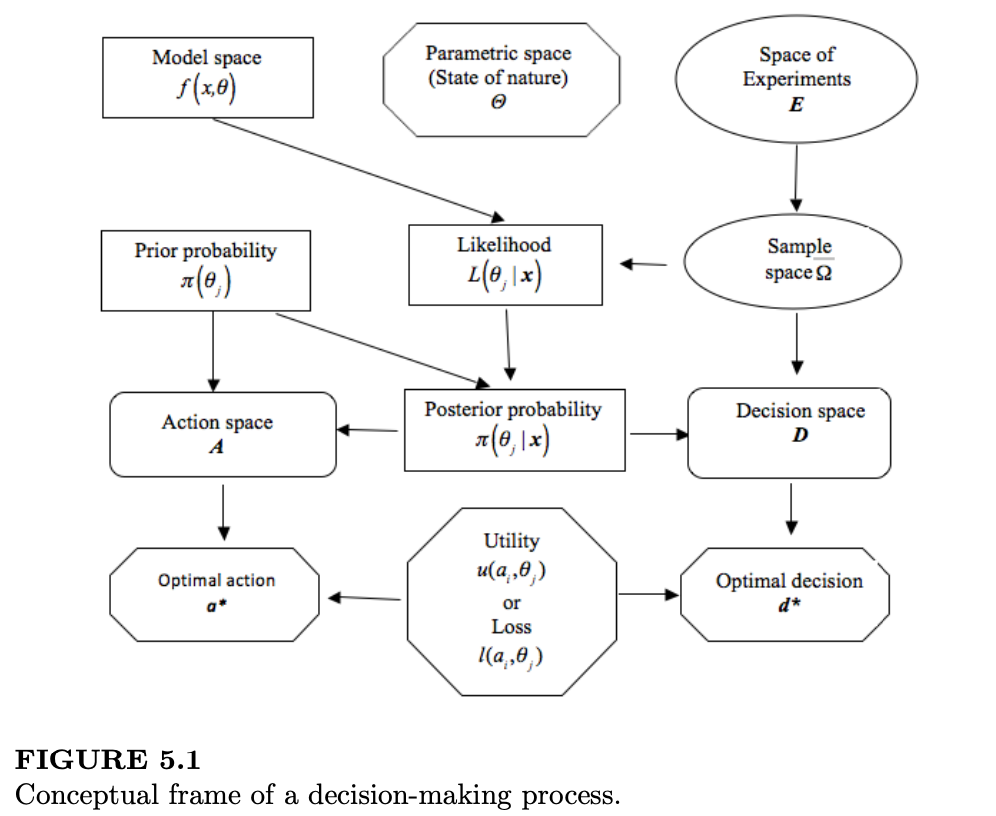
\includegraphics[width=\linewidth]{Images/SDTSchema.png}
	\caption{SDT Schema.}
	\label{fig:SDTScheme}
\end{figure}

The project (SDT authors call it a \textit{process}) is a sequence of states and actions (and sometimes decisions). To obtain the best performance out of the project a measure of utility instead of simple monetary reward can be introduced. The uncertainty in a project is addressed by a parameterized model with prior distribution that concentrates all knowledge relevant to the project. 

The best action strategy is the one that maximizes cumulative utility and it is usually obtained by a method of backward induction called dynamic programming. 

\begin{definition}
	TODO - a proper definition of dynamic programming. 
\end{definition}

Not sure about what is the difference between stochastic decision theory and stochastic control theory. They are probably synonyms. 

Dynamic programming is a tool used for determining the optimal strategy and a value of a project (\textit{process}). Its core is the Bellman equation, which represents the backward induction of value function computation. 

Real option analysis can be understood in multiple ways. If a replicating portfolio exists, then a value of some expected cash flow is identical to the current value of a portfolio. The support for this statement comes from the law of one price from economics. The assumption of replicating portfolio existence becomes hard to defend as the project that is to be valued becomes more abstract and/or complex.

For more complex projects, real option valuation uses binomial models with risk-neutral probabilities coming from the law of one price (Guthrie \cite{Gut:09}), or stochastic models of an expected behavior of the state variable determining the future cash flow (Vollert \cite{Vol:03}). 

\section{My valuation}
This sub-chapter is my attempt to best describe a real option valuation understood in a sense of an opportunity to make change in future project's cash flows. 

First I start with the intuitive equation: 

\begin{equation}\label{eq:valIntuitive2}
	V = \max_{\pi \in \mathbf{\Pi}} E\left[\sum_{t \in \mathbf{T}} DC_t(s_t,b_t(\pi)) \right], 
\end{equation}
where $\pi $ is a strategy, a sequence of decisions that the manager is able to do to change the course of the project. Time evolution of the process is represented by a variable $t$ which iterates over range of time epochs, so far finite or infinite countable $\mathbf{T}$. Discounted cash flow $DC_t$ assumed to be obtained at the end of an epoch $t$  is derived from the free cash flow $C_t$ and a constant discount rate $r>1$ as: 

\begin{equation}\label{eq:discCF2}
	DC_t = \frac{C_t}{r^t}. 
\end{equation}


\begin{assumption}
	Discount parameter is constant in time. 
\end{assumption}
 We can see that $DC_t$ depends on two variables, state variable $s_t$, which represents the state of an environment (outer world, like prices of oil, price of skilled software engineers, etc.) and $b_t$, project "branch", which represents that state of the project itself (inner property of the project, for example if a copper mine is active or idle, or if the decision was to produce chocolate instead of vanilla ice cream). 
 
 \begin{assumption}\label{ass:independence}
 	State variable $s_t$ is a random variable and does not depend on actions of the project's management. 
 \end{assumption}

Assumption \ref{ass:independence} can be violated for example in duopolistic markets or others, where a single company decision has non-negligible influence on the market. 

\begin{assumption}\label{ass:branchVar}
	A "branch" upon which the project is in the moment is assumed to be a random variable and  its value is determined only by actions in a policy $\pi$ and its random nature. 
\end{assumption}

Assumption \ref{ass:branchVar} is reasonable for majority of projects. Management makes a decision to open or close a mine, to produce chocolate or vanilla. However, for example in some R\&D projects the outcome of a manager's decision is uncertain. 

\subsection{Addressing the uncertainty}\label{subs:addressingUncertainty}
In this subsection the meaning of the expected value will be examined. We follow on the equation \ref{eq:valIntuitive} \footnote{not sure about the expression}. Using the linear property of expectation $E$ and substituting for $DC_t$ with equation \ref{eq:discCF} we obtain: 

\begin{equation}
	V= \max_{\pi \in \mathbf{\Pi}}\sum_{t \in \mathbf{T}}\frac{E[C_t(s_t,b_t(\pi))]}{r^t}.
\end{equation}

\begin{assumption}
	Environment $s_t$ can take on values from a finite or countable set $\mathbf{S_t}, \forall t \in \mathbf{T}$. 
\end{assumption}

This assumption is important only for simpler discussion later. Uncountable $\mathbf{S_t}$ could probably work too, but we would need to perform integration instead of summation \footnote{The verb integrate probably has a different meaning. }. 

 \begin{assumption}\label{ass:branchState}
	The actual state of $b_t \in \mathbf{B_t}$ depends only on actions in policy $\pi$ that happened before the time period $t \in \mathbf{T}$. 
\end{assumption}

As a result of assumption \ref{ass:branchState} a term \textit{partial strategy} is defined. 
\begin{definition}\label{def:partialStrategy}
 A partial strategy $\pi_t$ for a full strategy $\pi$ is defined as the first $t$ elements of its vector, $\pi_t = (a_1,a_2,..., a_t)$\footnote{It can be noticed that $\pi_{|\mathbf{T}=\pi}$}.
\end{definition}


\begin{assumption}
	For a given partial strategy $\pi_t$, the project "branch" can take on values from a finite set $\mathbf{B_t}, \forall t \in \mathbf{T}$. 
\end{assumption}

In most cases the "branch" of a project is a deterministic function of a managerial decision, however $b_t$ also covers variables whose evolution is triggered by a managerial decision. For example building a bridge with toll payments a year later also postpones the "adoption curve" of the new road. 

\begin{assumption}\label{ass:bsIndep}
	The state of an environment $s_t$ and the branch state $b_t$ are stochastically independent random variables. 
\end{assumption}
Using assumptions \ref{ass:branchState}, \ref{ass:bsIndep} and definition \ref{def:partialStrategy} we arrive at the final valuation formula:

\begin{equation}\label{eq:valuationFinal}
	V= \max_{\pi_{t-1} \in \mathbf{\Pi}}\sum_{t \in \mathbf{T}}\frac{\sum\limits_{s_t \in \mathbf{S_t} } \sum\limits_{b_t \in \mathbf{B_t}(\pi_{t-1}) }p(s_t)p(b_t(\pi_{t-1}))C_t(s_t,b_t(\pi_{t-1}))}{r^t}. 
\end{equation}

 Now, there are several questions about our ability to actually compute this valuation. 

\begin{itemize}
	\item Where do the sets $\mathbf{T}, \mathbf{S_t}, \mathbf{B_t}$ come from? 
	\item How to determine the discount factor $r$. 
	\item How are we able to obtain the cash flow function $C_t(s_t, b_t)$?
	\item What are we maximizing over? What is the set of possible strategies $\pi \in \Pi$?
	\item How to obtain the probabilities $p(s_t), p(b_t(\pi_{t-1}))$?
\end{itemize}

All of these questions will be answered in the next section. 

\subsection{Actual value computation}
In this section we will be discussing, how to actually value a project with the equation \ref{eq:valuationFinal}.
\subsubsection{Sets $\mathbf{T}, \mathbf{S_t}, \mathbf{B_t}$}
All of the sets $\mathbf{T}, \mathbf{S_t}, \mathbf{B_t}$ come from the model of a valuation problem.
 
 The number and frequency of time periods is determined by $\mathbf{T}$, when the most usual approach is to have $\mathbf{T}$ as a finite number of yearly periods. This can represent either a duration of project rights (for example in mining) or rights for a cash flow share (for example from bridge tolls), or such fuzzy future, where nobody really knows what will happen with the project 50 years from now. 
 
 The set of possible branches $\mathbf{B_t}$ comes from the project manager. He needs to identify the project alteration possibilities in each time period $t \in \mathbf{T}$. The set $\mathbf{B_t}$ is small most of the time, however in cases, when for example a start of a variable that is modeled by binomial tree is dependent on the strategy, the set $\mathbf{B_t}$ can grow rather quickly. The example is again a bridge project, where the number of toll-paying customers in time $t$ depends on a time period in which the bridge was finished. 

 
 And finally, the values of an environment state $\mathbf{S_t}$ are determined by a model of the outer world. The set $\mathbf{S_t}$ should be able to capture the uncertainty about all important parameters for the project while remaining as simple as possible. A classical example is a binomial tree of input prices for our process (oil, software engineer's salary).
 
 \subsubsection{Discount factor $r$}
 The discount factor, representing time value of money plays a big role in the financial world. It is expected to be $r>1$ because today's economy depends on non-negative inflation. 
 
 \begin{assumption}\label{ass:discountFactor}
 	The discount factor $r$ is expected to be larger than one and constant through the project's lifetime. 
 \end{assumption}
The assumption \ref{ass:discountFactor} serves as a simplification. To study time variant discount factor in the light of real option valuation is not interesting. However, one could simply model the discount rate as $r_t$ with some probabilities $p(r_t)$ and compute an expected discount rate. 
 
 \subsubsection{Cash flow function}
 The core of each project valuation is its cash flow function $C_t(s_t,b_t)$, which represents the additional monetary value created by it over some time period. Usually, this function is simply defined as the difference between the total price of inputs (usually given by $s_t$) and outputs (usually given by $b_t$ or $s_t$) for a given period. In more complex models, the inputs can also represent depreciation of machinery, expenses on marketing campaigns or additional costs to acquiring new workforce (not only their salary).
 
 An example of zero cash flow is when a project is deferred and waits to be undertaken or not. A simple example of non-zero cash flow is a project of running ammonia factory, where the cash flow is:


 \begin{equation}
 	C_t = \frac{n_g}{c_{g\rightarrow a}}p_a - n_g*p_g, 
 \end{equation}
 where $n_g$ is the volume of processed gas, $p_g, p_a$ are prices of gas and ammonia on the market and $c_{g\rightarrow a}$ is an inner company coefficient, that says how many units of gas are needed to produce one unit of ammonia. 
 
 \subsubsection{Strategies $\pi$}
 As was pointed out by many articles \footnote{See for example \cite{}, \cite{}, or \cite{}.} the ability to change the course of a project has value. The sequence of actions (in some papers called decisions) form a strategy $\pi = (a_1, a_2,..., a_{|\mathbf{T}|})$. 
 
 \begin{assumption}
 Action $a_t$ is expected to happen in the end of the corresponding time period $t \in \mathbf{T}$. 
 \end{assumption}

The set of possible strategies $\mathbf{\Pi}$ needs to be given by a manger responsible for the project or his team. He should know best, what are the possible changes in the project, that could improve its cash flow and increase its value. 

The set of possible strategies is usually well defined by a real options understood in a sense of an ability to act. 

In an example from \cite{Gut:09}, an operator of a gas power plant can choose to produce electricity or not to, based on the current price of gas and power. The strategies in this example can be represented as binary vectors: 
\begin{equation}
\mathbf{\Pi} = \{(a_1,...a_{|\mathbf{T}|})|a_i \in {1,0}, \forall i \in \mathbf{T}\}, 
\end{equation}
where $a_i = 1 $ means that the plant is running in the next time period $i+1$ and $a_i=0$ means that the power plant will be in an idle state. 


\subsubsection{Probabilities}
Finally, the most complex problem from the list in the end of section \ref{subs:addressingUncertainty} is to determine what to substitute all $p(s_t)$ and $p(b_t)$ in the equation \ref{eq:valuationFinal} for. 

The difference in the ROA, SDT and for example DTA techniques is mainly in the difference in which they cope with the derivation of these values. 

For DTA, both $p(s_t)$ and $p(b_t)$ are assumed to be known in each time period. This is because problems solved with DTA are usually simple and they need to declare only small number of probabilities. 
 
 For ROA the probabilities $p(s_t)$ arise as the so-called risk-free probabilities that come from the idea of replicating portfolio and the validity of the law of one price. For example Guthrie in \cite{Gut:09} uses the capital asset pricing model (CAPM), that provides risk-neutral probabilities of up and down movements, $p_u, p_d$. All other probabilities that could be defined as $p(s_t)$ are in \cite{Gut:09} determined by a binomial pricing model as a product of $p_u$ and $p_d$. 
 
 Another approach to ROA can be seen in the work of Vollert \cite{Vol:03}, who models the replicating portfolios as some stochastic Ito process, which gives the probabilities of $s_t$. 
 
The branch probabilities $p(b_t)$ are in ROA not understood as a separate category, thus they do not need to be further discussed\footnote{Not sure about this, check it. }. 
 
 
 Finally, in SDT, the value of both $p(s_t)$ and $p(b_t)$ comes from the knowledge about the underlying problem expressed as prior (or posterior, when updated for new data) probability distribution. The prior probability distribution is constructed from the inner knowledge of experts on the subject, former relevant data, principle of insufficient reasons or their combinations. In SDT it is usually expected that $p(s_t)$ comes from some parameterized family of distributions: 
 \begin{equation}
 	\mathcal{F} = \{p(s_t|\theta)|\theta \in \mathbf{\Theta} \}. 
 \end{equation}
 
 An example is a binomial distribution $Bi(t,\theta)$:
 \begin{equation}
  p(s_t = k|\theta) = \binom{t}{k}\theta^{k}(1-\theta)^{t-k}.
 \end{equation}
 
 I believe that this approach is the most general, because one can interpret the prior distribution in many possible ways. The SDT approach also allows for combination of many different sources of knowledge about the project \cite{}. 
 
 The problems of ROA approach are the inability to find a replicating portfolio to any more complex project and unclear and undiscussed origins of "actual" probabilities in CAPM model and other variables in it used in \cite{Gut:09}.
 
  The STD approach is protected against these problems, as even when there is no prior, there is always a principle of insufficient reasons, which needs only a model, a requirement of all techniques that try to determine $p(s_t)$ and $p(b_t)$.
 
 
 \subsection{The maximization process}
 
TODO after supervisor's review. In a nutshell it is a dynamic programming and after realization that the complexity is large, it is approximate dynamic programming.  
 
 \subsection{Note at the end}
 
 Without using the replicating portfolio, the "Real Options" in my workmeans only the ability to change the projects path as is presented in articles \cite{Cop:01},... I would love to incorporate the law of one price in the priors of SDT somehow. 
 
 






\chapter{Application of the cheery-picked valuation technique. }
The class of .... valuation problems is ideal for demonstration of the usability of the newly developed valuation technique. Due to the inherit uncertainty in this field and many actions that can be undertaken, the additional value  assigned to the investment opportunity can be significant. 

We start with a rigorous mathematical definition of this class of valuation techniques in terms of SDT. Then we pick one example and promptly show that the number of possible states is exponential with respect to... Approximate dynamic programming techniques like Q-learning or SARSA were developed in order to solve exactly these types of problems. Due to their strengths and only a minor flaws their usage is justified. 


 \section{Approximate dynamic programming}
<Proposal of a fitting method to the class of problems defined above> 

\section{Valuation example}
 
 \subsection{NPV valuation }
 
 \subsection{DTA valuation}
 
 \subsection{Classic ROA valuation}
 
 \subsection{New approach}
 


\chapter{Discussion}
The new approach is better because it solves the current problems with ... Also the applicability of the new approach is in my opinion broader since it can address multiple sources of uncertainty. Furthermore the power of the decision making process is kept in the hands of the decision maker through creation of prior distributions. The manager is guided through the world of utility functions and priors, which both can be created from a set of simple questions about gambles and beliefs of the manager. The creation and usage of the utility and prior density functions are fool-proof in a sense of mathematical coherence. 




\chapter{Conclusions}
In my master's thesis I have rigorously compared the state-of-the-art valuation techniques used in present investment companies. I have shown the advantages and disadvantages of real option analysis  and stochastic decision theory. The combination of these, which I call ...,  yields a new view on the world of risky investments that empowers the decision maker and thus allows for better adoption in the rigid environment of investing. 







\chapter{Bachelor's thesis parts that could be useful for TeX styling}




\section{Discrete Markov decisions processes}\label{DMDPSection}
A lot of real life decision tasks can be approximately described by the mathematical framework called discrete Markov decision processes (MDPs), Fig. XY. The definition of this mathematical framework is crucial for this work, as it is the basis upon which the theory of policy optimisation is built. 

\begin{definition}
	Discrete Markov Decision Process $\mathcal{M}$ is defined as ordered set of five elements $(\textbf{T},\textbf{S},\textbf{A},P,R) $, where:
	\begin{itemize}
		\item \textbf{T} stands for a discrete, finite set of decision epochs; $\textbf{T}=\{0,1,2,...,|\mathbf{T}|\}$, where\footnote{Because the number of time epochs $|\mathbf{T}|$ is used frequently, the notation $|\mathbf{T}|=N$ is used.} $|\mathbf{T}| \in \mathbb{N}$
		
		The state in time epoch $t=0$ is known and it is denoted $s_0$.
	\end{itemize} 
	
\end{definition}\label{DMDP}


\begin{definition}\label{ValueF} 
	Let $\mathcal{M}=(\textbf{T},\textbf{S},\textbf{A},P,R)$ be a MDP and $\pi_t \in \mathbf{\mathbf{\Pi_t}}$ a policy, then \textbf{value functions} of $\mathcal{M}$, $\varphi_{t}^{\pi_t}: \mathbf{S}\rightarrow \mathbb{R}$ are defined $\forall \pi_t \in \mathbf{\Pi_t}$, $\forall t \in \mathbf{T}\setminus \{N\}$ as:
	\begin{equation}
	\varphi_{t}^{\pi_t}(s)=E\bigg[\sum_{\tau > t, \tau \in \mathbf{T}}R(s_\tau,a_{\tau-1},s_{\tau-1})\big|s_t=s\bigg], 	
	\end{equation}
	
\end{definition}


\begin{theorem}\label{DynProgTheo}
	Let $\mathcal{M}=(\textbf{T},\textbf{S},\textbf{A},P,R)$ be a MDP, then the optimal value function $\varphi_t^{o}(s)=\max_{\pi_t \in \mathbf{\Pi_{t}}}\varphi_t^{\pi_t}$ can be computed recursively $\forall t \in \mathbf{T}\setminus\{N\}$ through the equation:
	
	\begin{equation}
	\varphi_t^{o}(s)=\max_{a_t \in \mathbf{A}} E\bigg[R(s_{t+1},a,s) + \varphi_{t+1}^{o}(s_{t+1})|a_t,s\bigg],
	\label{DynProgEq}
	\end{equation}
	considering that $\varphi_{N}^{o}=0$ as Definition \ref{ValueF} implies. Furthermore the optimal policy $\pi_{t}^{o}$, as the argument of maxima, is concentrated on maximising arguments in Equation (\ref{DynProgEq}). 
	
\end{theorem}

\begin{proof}
	This theorem will be proven via a finite backward mathematical induction.
	
	At first, let us take an action $a^{o}_{N-1}$ in the time epoch $N-1$ defined as:
	\begin{equation}
	a^{o}_{N-1}(s) = \mathrm{Arg}\max_{a\in\mathbf{A}} E[R(s_{N},a,s)|a,s].
	\end{equation}
	By the definition of maxima the inequality
	
\end{proof}


We can now describe the dynamic programming algorithm in detail.

\begin{algorithm}
	\caption{Finding the optimal policy for a \textit{single system} MDP with known $P$}\label{alg:SingleKnown}
	\begin{algorithmic}[1]
		\Require{$\mathcal{M}=(\textbf{T},\textbf{S},\textbf{A},P,R)$}
		\State$ \varphi_N^{o}(s) \gets 0$, $\forall s \in \mathbf{S} $ \Comment{Based on Definition \ref{ValueF}.}
		\State $t \gets N$ 
		\While{$t\ne 0$}
		\For{ each $s \in \{1,2,...,|\mathbf{S}|\}$}
		\State $\varphi_{t-1}^{o}(s) \gets Equation$ $(\ref{DynProgEq})$ \Comment{With known $P$ and $\varphi_{t}^{o}$}
		\EndFor
		\State $t \gets t-1$
		\EndWhile
		\State $\pi_{0}^{o}(s) \gets argmax$ $\varphi_0^{o}(s)$ $ \forall s\in \mathbf{S}$, \Comment{Deriving the optimal policy}
		\State	\Return{$\pi_{0}^{o}$}
	\end{algorithmic}
\end{algorithm}




\begin{example}\label{Ex:Multi}
A real life example of this MDP could be again a biased coin tossing. Imagine a game when you are sitting at the table on which there are multiple coins with generally different bias. You get one coin on certain side in your hands and you are told the rules. You get $\$$1 each time the coin lands on Heads. You can choose to change your coin for any other coin for $\$$3 and you have to place it to the side it is on the table (you have to "conserve its state"). The turn of the coin costs 5 cents and the result of the toss generally depends on the side from which the coin is tossed. You know the bias of each one coin and the question is: what is the best sequence of actions that you can perform to get as much money as possible, on average, from this $N$-round game?

It is important to mention that you are able to see the other coins "on the table" so that the position state $s^{p}$ is known in each time epoch. 
\end{example}



\paragraph{Discussion}
The main goal of this simulation is to check the quality of the experimentally derived sub-optimal policy via Algorithm \ref{alg:SingleKnown}. As we can see, the difference between the average cumulative reward of the derived policy and the expected optimal average cumulative reward is approximately $0.5\%$ in the first simulation with 500 Monte Carlo iterations and approximately $0.026 \%$ in the second simulation with 5000 iterations.  \footnote{I dont know how to fit the exceedance in here, so if it is not that important I would prefer not to talk about it.}

We can also see that in the second performed experiment made for 5 000 iterations, ten times the first case, both the variance of the distribution and the difference from the optimal value decreased. It is then assumed that this trend would continue with more iterations and that both the variance and the difference would get closer and closer to zero.

With this assumption we can say that the experimentally derived optimal policy is in fact the optimal one. \footnote{Is that a good reasoning?}




\begin{table}[H]
	\centering
	\renewcommand{\arraystretch}{2}
	
	
	\begin{tabular}[t]{|r|r |r|}
		\hline
		\multicolumn{3}{|c|}{$P(:,:,s=1)$} \\
		\hline
		$\tilde{s}$/$a$  & 1 & 2\\
		\hline
		1	& 0.4237&	0.6885\\
		\hline
		2 & 0.5763 & 0.3115 \\ 
		\hline
		
		\multicolumn{3}{c}{} \\[-0.4cm]
		\hline
		\multicolumn{3}{|c|}{$P(:,:,s=2)$} \\
		\hline
		$\tilde{s}$/$a$ & 1 & 2\\
		\hline
		1	& 0.7282&	0.8816\\
		\hline
		2 & 0.2718 & 0.1184 \\ 
		\hline
	\end{tabular}
	\hfill
	\begin{tabular}[t]{|r|r |r|}
		\hline
		\multicolumn{3}{|c|}{$R(:,:,s=1)$} \\
		\hline
		$\tilde{s}$/$a$  & 1 & 2\\
		\hline
		1	& 1.4315&	-0.0569\\
		\hline
		2 & 2.7287 & -0.3111 \\ 
		\hline
		
		\multicolumn{3}{c}{} \\[-0.4cm]
		\hline
		\multicolumn{3}{|c|}{$R(:,:,s=2)$} \\
		\hline
		$\tilde{s}$/$a$ & 1 & 2\\
		\hline
		1	& -0.1039&	2.5921\\
		\hline
		2 & 1.1251 & -0.2876 \\ 
		\hline
	\end{tabular}
	\hfill
	\begin{tabular}[t]{|r|r |r|}
		\hline
		\multicolumn{3}{|c|}{$w(:,:,s=1)$} \\
		\hline
		$\tilde{s}$/$a$  & 1 & 2\\
		\hline
		1	& 8&	5\\
		\hline
		2 & 1 & 2 \\ 
		\hline
		
		\multicolumn{3}{c}{} \\[-0.4cm]
		\hline
		\multicolumn{3}{|c|}{$w(:,:,s=2)$} \\
		\hline
		$\tilde{s}$/$a$ & 1 & 2\\
		\hline
		1	& 1&	2\\
		\hline
		2 & 9 & 1 \\ 
		\hline
	\end{tabular}
	\caption{Tables of $P$, $R$ and $w$ values for the CE approach simulation. Original 3D arrays are presented by two  "slices" which differ in the initial state $s=1$ or $s=2$. }\label{Tab:PRwValues}
\end{table}\footnote{Hope this representation is OK, and how to do the backslash $\tilde{s},a$?}


\pagestyle{plain}

\bibliographystyle{plain}

\bibliography{fr}




\end{document}
